\section{How did you meet your spouse? When did you know you wanted to marry them?}
Well, we met during high school and knew of each other, but it was more than seven years later that we connected with each other.
I was teaching at New Danville School with Barb, John's sister.
Several of the teachers started a bible study/discussion group.
John started coming to that group.
We got to know each other as participants in the group.
I was at a time in my life that I was feeling good about living the single life.
John and his friend Chris took off for a several week tour of Europe.
Summer turned to fall and then winter.
I was planning to spend Christmas with one of my housemates in Indiana with her family.
On December 16 some of the group we were part of got tickets to hear Handel's Messiah sung at the Fulton Opera house in Duke Street in Lancaster.
\begin{figure}
\centering
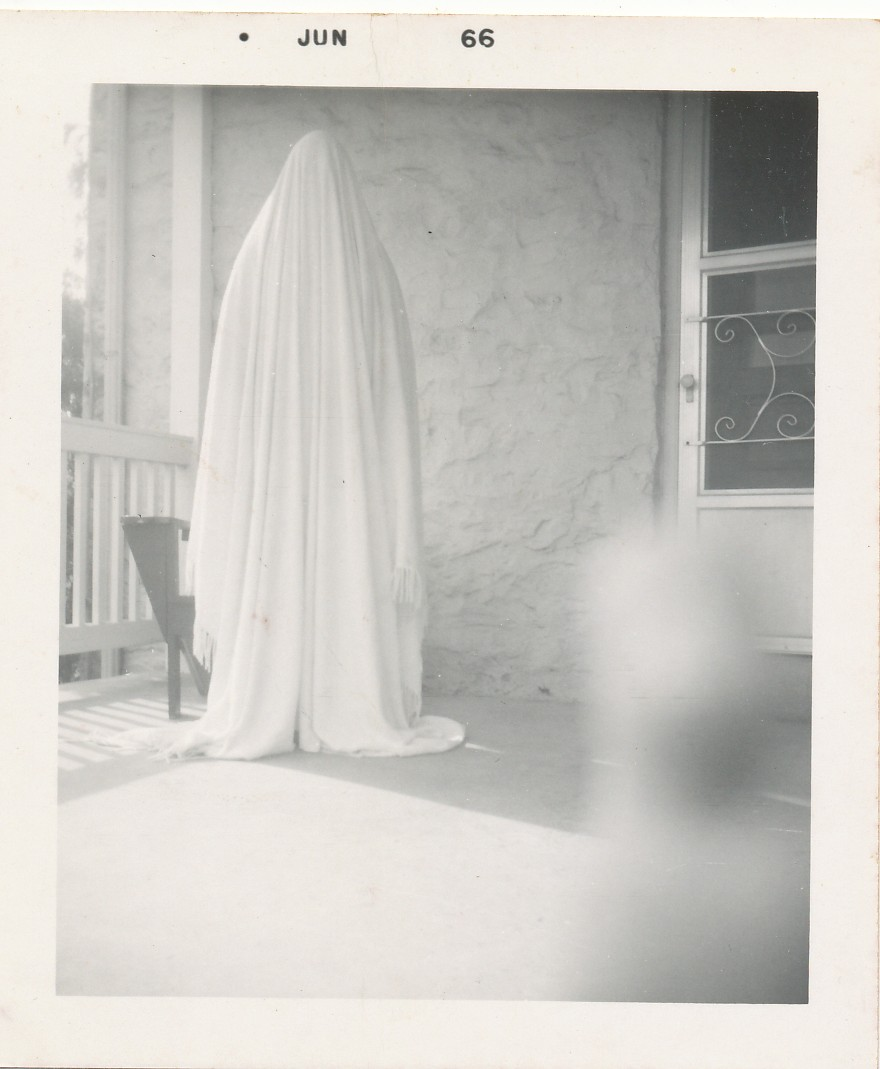
\includegraphics[width=0.9\textwidth]{marriage/1.jpg}
\caption{
My ticket for the concert the night John asked me if I'd be interested in dating.
}
\end{figure}

I offered to drive and pick up some other people.
One of the people was handicapped so I left the group off and then found parking for my car.
I was a fine evening with good music.
As I left to bring the car to pick up my friend, John asked if he could come with me.
I said fine no problem.
We were in the car driving back to pick up the rest of the group when John said that he would be interested in dating.
I was floored to say the least.
I did not know what to say.
Since I did not say anything he was concerned that I was going to reply negatively.
I was not feeling negative about his request, I just didn't know what to say.
I must have responded positively because we did begin dating.
This change in situation was a shock to my system and my two housemates teased me.
Our first date was Christmas caroling with the folks at River Corner Church.
Then I spent Christmas in Indiana.
I was back in time for my family gathering on New Year's weekend.
John worked on Saturdays so I thought I could ask him to the family gathering and he would decline.
However, he decided to get off work and come to the Hess gathering and we had had only two dates.
What would my family think?
Well they took this as a sign that this was a serious relationship since the pattern was that once someone brought a "friend" to a family gathering they were likely to get married.
There was no small pressure there.
\begin{figure}
\centering
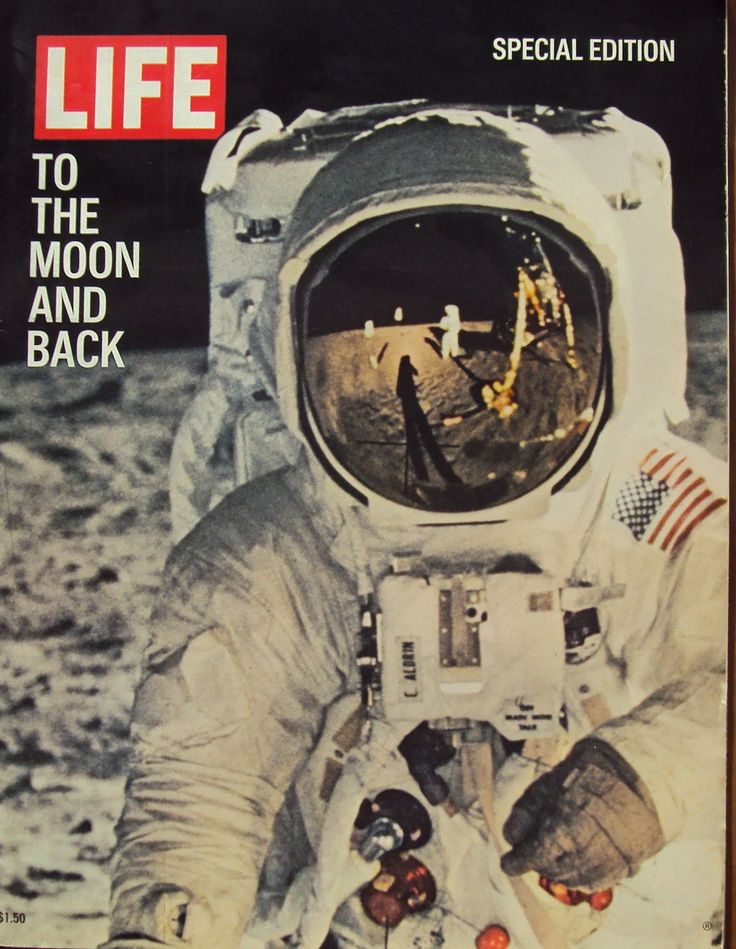
\includegraphics[width=0.9\textwidth]{marriage/2.jpg}
\caption{
Friends, Sandy and Martin at my family gathering
}
\end{figure}

So the days and weeks went by.
Not a week passed that we did not spend time together.
I met his family.
I was applying for a new job at Locust Grove School.
It was for a new program where I would work one on one with student who have learning disabilities.
It required two weeks of training in Norfolk, VA during the summer.
As I filled out the application in April I came to a question I did not know how to answer.
Do you have or might you have plans to get married during the next year.
What a question! It could not be asked on an application today.
But what was I to do? I could not in all fairness answer this by myself since I was now in relationship with John.
So I showed him the question.
He said - why not! He was heading toward student teaching in the fall semester and liked the idea of being married during that time that can be rather stressful.
So we got engaged on April 16, four months after John told me he was interested in dating.
\begin{figure}
\centering
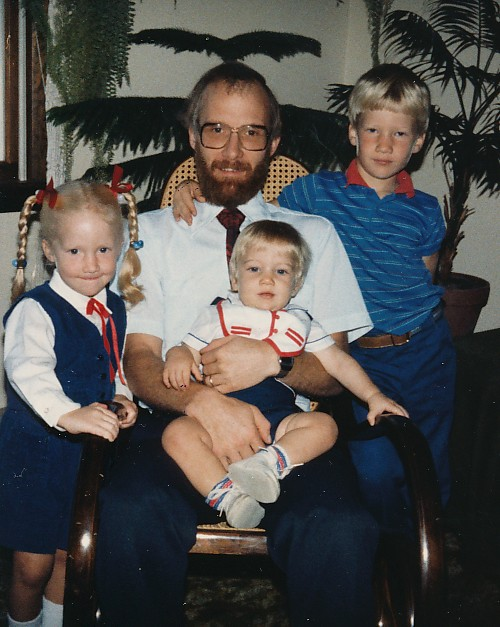
\includegraphics[width=0.9\textwidth]{marriage/3.jpg}
\caption{
Engaged - Facing the Future Together
}
\end{figure}
There was a lot to do in the next four months since we decided to get married on August 26.
\begin{figure}
\centering
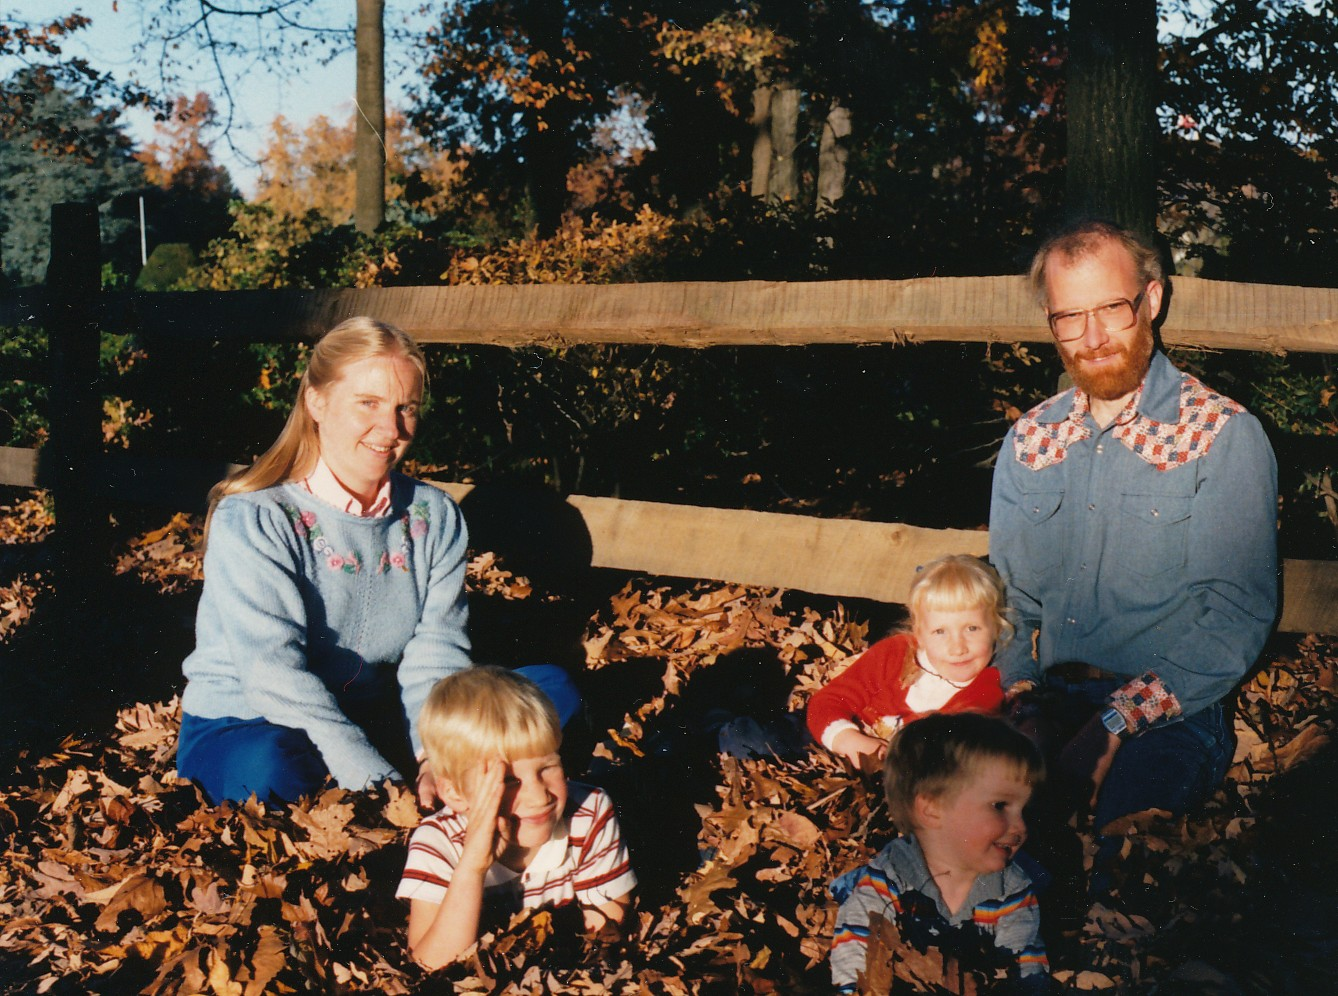
\includegraphics[width=0.9\textwidth]{marriage/4.jpg}
\caption{
Engagement announcement
}
\end{figure}
We chose to get married on a Sunday at the Hans Herr House, the only day of the week the place was closed to the public.
\begin{figure}
\centering
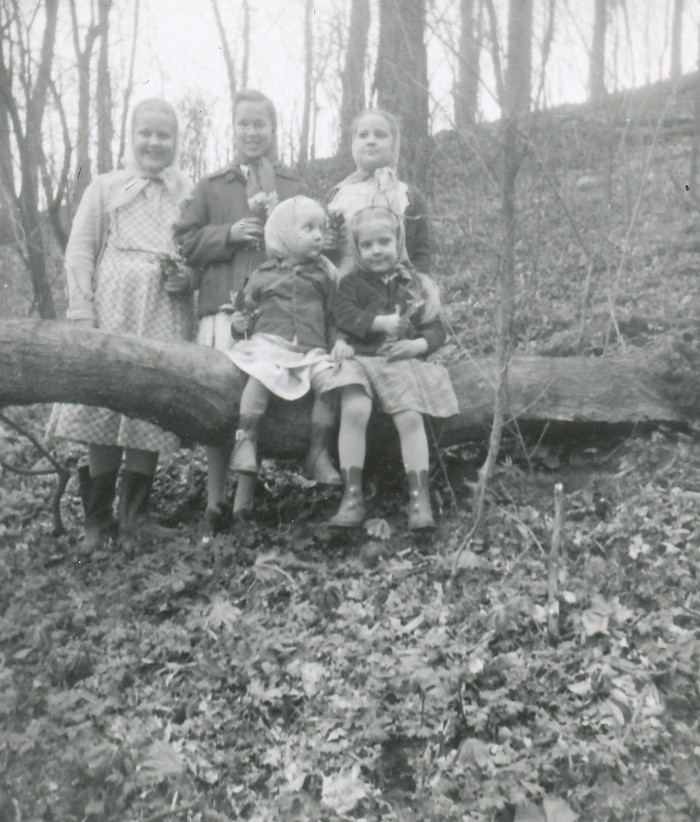
\includegraphics[width=0.9\textwidth]{marriage/5.jpg}
\caption{
Our wedding day at the Hans Herr House, August 26th 1979
}
\end{figure}
I along with Sandi Harnish and Rose Kennel were living in the apartment above the visitor's center of this lovely historic place.
We got married under the trees on a warm hazy August day and left for a trip to New England.
We returned in less than a week and moved into an upstairs apartment in Millersville.
\begin{figure}
\centering
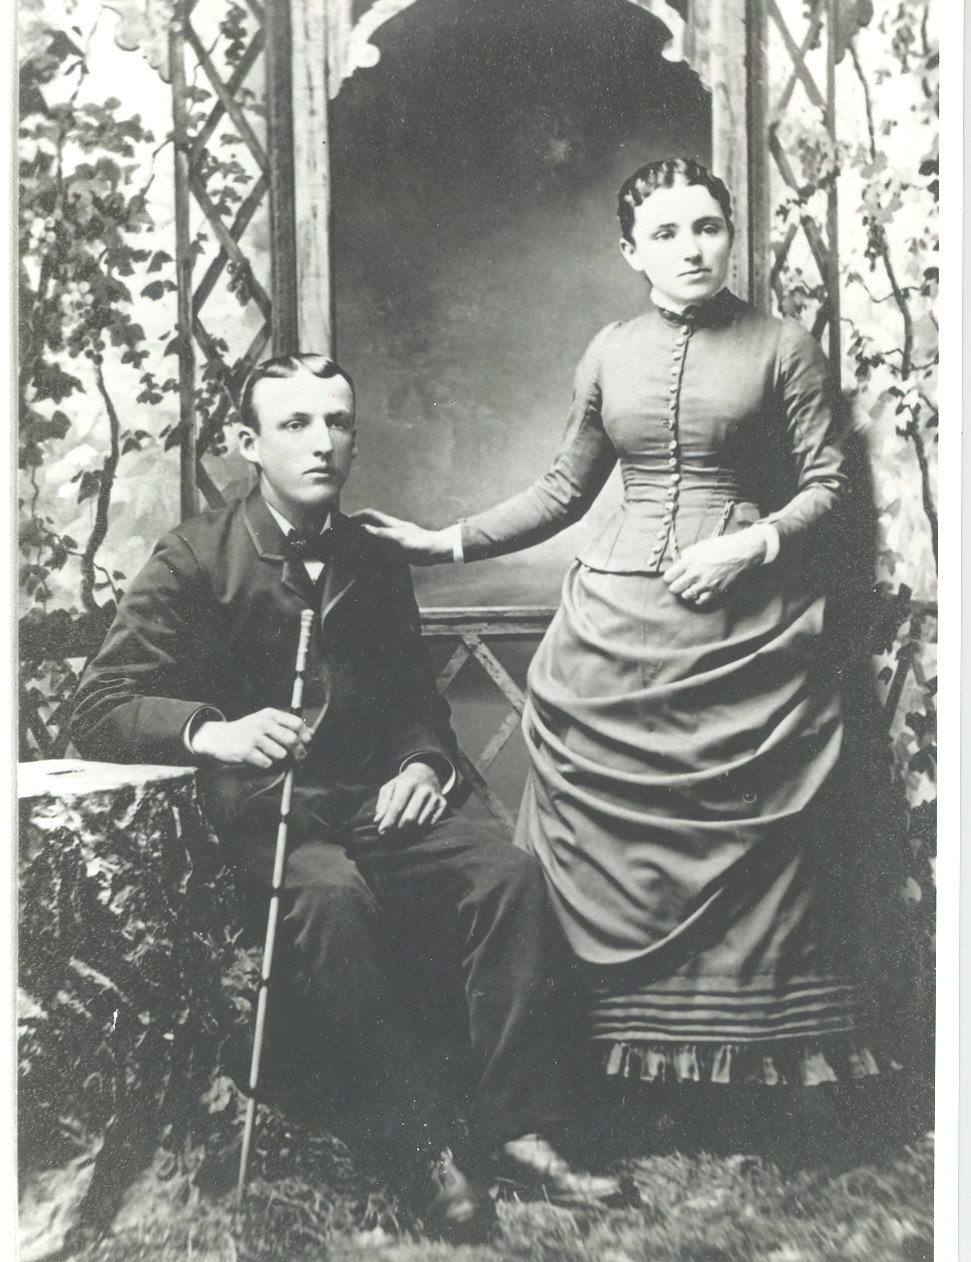
\includegraphics[width=0.9\textwidth]{marriage/6.jpg}
\caption{
Wedding announcement
}
\end{figure}
